% Appendix A

\chapter{Costruzione di $\mathcal{Z}$}

\definecolor{main-color}{rgb}{0.6627, 0.7176, 0.7764}
\definecolor{back-color}{rgb}{0.1686, 0.1686, 0.1686}
\definecolor{string-color}{rgb}{0.3333, 0.5254, 0.345}
\definecolor{key-color}{rgb}{0.8, 0.47, 0.196}
\definecolor{myblue}{rgb}{0.117647 0.564706 1}
\definecolor{codegreen}{rgb}{0,0.6,0}


\lstdefinestyle{mystyle}{
	 framexleftmargin=6pt,
	framextopmargin=6pt,
	framexbottommargin=6pt, 
	frame=tb, framerule=0pt,
	language = SQL,
	basicstyle = {\color{main-color}},
	backgroundcolor = {\color{back-color}},
	commentstyle=\color{codegreen},
	stringstyle = {\color{string-color}},
	keywordstyle = {\color{key-color}},
	keywordstyle = [2]{\color{red}},
	keywordstyle = [3]{\color{teal}},
	keywordstyle = [4]{\color{myblue}},
	otherkeywords = {PER, PERFORM, REPLACE, function, returns, void, DECLARE, BEGIN, LOOP, IF, FOR, LANGUAGE, FUNCTION, RETURNS, TEMP, TRUNCATE, WHILE, if},
	morekeywords = [2]{RECORD, geometry, SERIAL},
	morekeywords = [3]{\$\$},
	morekeywords = [4]{ST_Intersects, ST_Intersection, ST_Buffer, st_intersection, st_geometrytype, st_dump, st_linemerge, st_collectionextract, st_split, st_area, ST_Perimeter, st_centroid, st_x, st_y, regr_slope, st_makepoint, st_makeline, st_setsrid, st_distance, ST_LineSubString, st_lineinterpolatepoint, st_length},
	numberstyle=\normalfont\footnotesize\color{black},
	stepnumber=1,
	tabsize=2,
	literate=
	{á}{{\'a}}1 {é}{{\'e}}1 {í}{{\'i}}1 {ó}{{\'o}}1 {ú}{{\'u}}1
	{Á}{{\'A}}1 {É}{{\'E}}1 {Í}{{\'I}}1 {Ó}{{\'O}}1 {Ú}{{\'U}}1
	{à}{{\`a}}1 {è}{{\`e}}1 {ì}{{\`i}}1 {ò}{{\`o}}1 {ù}{{\`u}}1
	{À}{{\`A}}1 {È}{{\'E}}1 {Ì}{{\`I}}1 {Ò}{{\`O}}1 {Ù}{{\`U}}1
	{ä}{{\"a}}1 {ë}{{\"e}}1 {ï}{{\"i}}1 {ö}{{\"o}}1 {ü}{{\"u}}1
	{Ä}{{\"A}}1 {Ë}{{\"E}}1 {Ï}{{\"I}}1 {Ö}{{\"O}}1 {Ü}{{\"U}}1
	{â}{{\^a}}1 {ê}{{\^e}}1 {î}{{\^i}}1 {ô}{{\^o}}1 {û}{{\^u}}1
	{Â}{{\^A}}1 {Ê}{{\^E}}1 {Î}{{\^I}}1 {Ô}{{\^O}}1 {Û}{{\^U}}1
	{œ}{{\oe}}1 {Œ}{{\OE}}1 {æ}{{\ae}}1 {Æ}{{\AE}}1 {ß}{{\ss}}1
	{ű}{{\H{u}}}1 {Ű}{{\H{U}}}1 {ő}{{\H{o}}}1 {Ő}{{\H{O}}}1
	{ç}{{\c c}}1 {Ç}{{\c C}}1 {ø}{{\o}}1 {å}{{\r a}}1 {Å}{{\r A}}1
	{€}{{\euro}}1 {£}{{\pounds}}1 {«}{{\guillemotleft}}1
	{»}{{\guillemotright}}1 {ñ}{{\~n}}1 {Ñ}{{\~N}}1 {¿}{{?`}}1
}

Per la soluzione del problema in esame è indispensabile avere una partizione completa del territorio abruzzese in cui ogni \textit{Zone} ha associata un $Sz_k$ che ne indica la propensione alla frana (definizione \ref{def:zones}). Notoriamente i dati geografici non sono facilmente reperibili. In particolare per la regione Abruzzo non è stato mai effettuato uno studio sul campo per censire le aree esposte al rischio frana. Difficilmente un lavoro del genere (lungo e costoso) verrà mai finanziato. Non avendo quindi a disposizione questi dati è stato costruito un dataset sintetico che si ottiene incrociando tra loro diverse tipologie di dati al fine di ottenere l'informazione desiderata (il più possibile coerente con la realtà).\newline In questo caso specifico i valori di $Sz_k$ dovrebbero essere calcolati a partire dai dati territoriali delle singole variabili (tipologia di terreno, pendenza, presenza di vegetazione ecc) che contribuiscono ai fenomeni franosi. Più variabili sono presenti come dati di input, più il valore $Sz_k$ descriverà meglio l'esposizione al rischio. Il caso limite è quello di avere a disposizione tutti i dati relativi alle variabili dai quali estrapolare una stima che sia identica alla valutazione di un geologo. Il vantaggio di avere un unico parametro $Sz_k$ permette, nel caso in cui esso debba essere ricalcolato per via della disponibilità di nuovi dati, di lasciare invariato l'algoritmo. Tale approccio evidenzia quindi la robustezza del metodo proposto. Sulla base di queste considerazioni per costruire il dataset $\mathcal{Z}$ sono state necessarie tre iterazioni.

\subsection{\textbf{Iterazione 1}}
E' stata creata una griglia, di quadratini di lato l, di dimensioni $n*n$ in grado di contenere l'intera  $\mathcal{GEOAREA}$ (definizione \ref{def:geoarea}) dell'Abruzzo. La griglia è stata creata grazie ad una primitiva chiamata \textit{st\_createfishnet}. Questa primitiva è stata introdotta dalla comunità in quanto non presente nella versione base di PostGIS \cite{fishnet}. Essa nasce dall'esigenza di dividere un'area in aree più piccole tutte di forma quadrata ed analizzabili quindi in modo indipendente dalla geometria iniziale. Tale griglia è stata intersecata con la  $\mathcal{GEOAREA}$ (Figura \ref{fig:griglia}) per ottenere il partizionamento completo (Figura \ref{fig:abruzzoGriglia}). Questa operazione ha permesso di avere il territorio abruzzese diviso in tante \textit{Zones} descritte ognuna di esse da una geometria (poligono). Non è possibile garantire in questo modo un'area minima per le \textit{Zones}. Ciò accade esclusivamente lungo i bordi della 
$\mathcal{GEOAREA}$. 
\begin{figure}[h]
	\hspace{0.05\linewidth}
	\begin{minipage}[t]{0.40\linewidth}
		\centering
		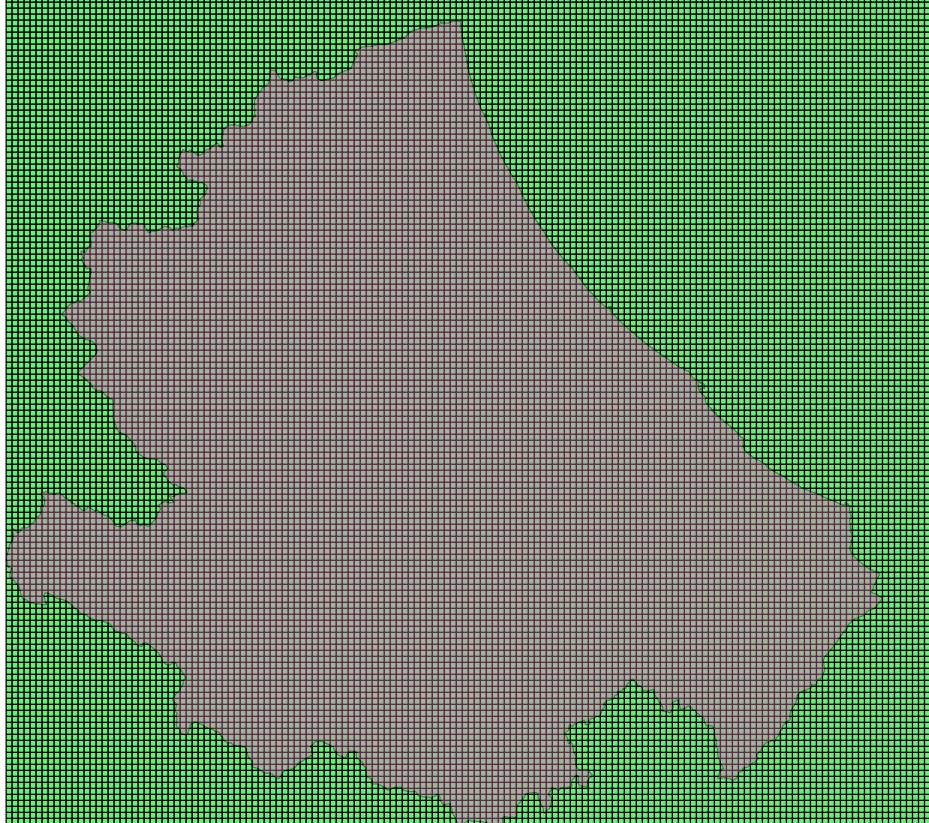
\includegraphics[width=\textwidth]{images/abruzzoQuadratini.PNG}
		\caption{In verde la griglia }
		\label{fig:griglia}
	\end{minipage}
	\hspace{0.1\linewidth}
	\begin{minipage}[t]{0.40\linewidth}
		\centering
		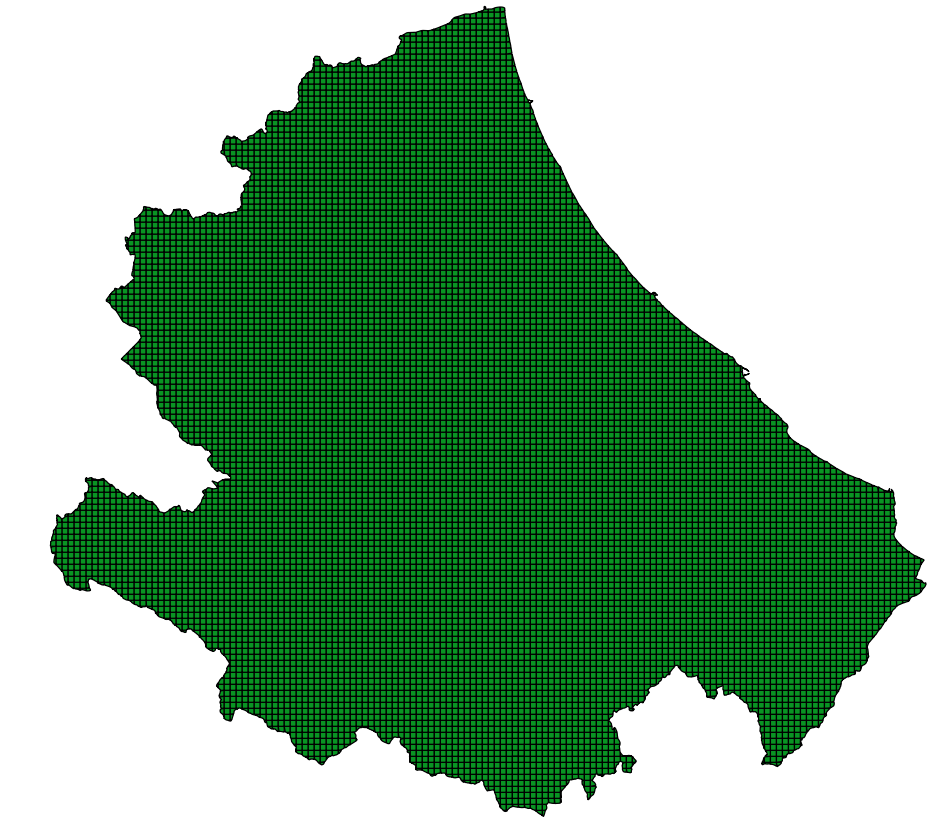
\includegraphics[width=\textwidth]{images/abruzzo.PNG}
		\caption{Risultato dell'intersezione.}
		\label{fig:abruzzoGriglia}
	\end{minipage}
\end{figure}

In questa iterazione è stato assegnato un valore di \textit{$Sz_k$} casuale (Figura \ref{fig:abruzzo_random}). 

\begin{figure}[H]
	\centering
	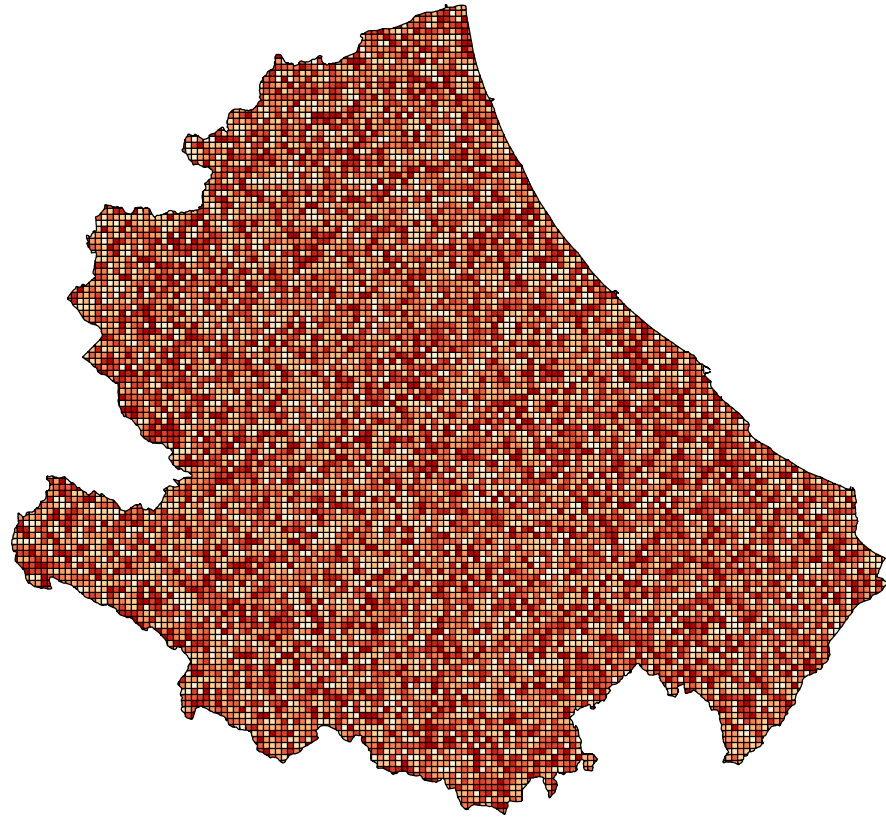
\includegraphics[width=0.8\textwidth]{images/AbruzzoRandom}
	\caption{Abruzzo partizionato con valore casuale di $Sz_k$}
	\label{fig:abruzzo_random}
\end{figure}


\subsection{\textbf{Iterazione 2}}
Assegnando valori $Sz_k$ casuali non si instaura una corrispondenza tra la morfologia del territorio e il dataset $\mathcal{Z}$. Per questo motivo qualsiasi risultato ottenuto, con il metodo proposto, sarebbe stato impossibile da validare in quanto viene a mancare un confronto tra i risultati prodotti dal metodo e quelli verificati sul campo da un team di esperti.    
Si è quindi deciso che tale valore doveva essere stimato secondo una logica ben precisa.
Non avendo uno studio geologico completo di tutto il territorio abruzzese si è presa in  considerazione una sola variabile tra quelle che contribuiscono al verificarsi di un evento franoso (Capitolo \ref{ch:introduction}) ovvero la pendenza del suolo. 
Sono state quindi introdotte le curve di livello. Esse rappresentano tutti i punti a stessa quota sul territorio. Le curve di livello  sono state ottenute a partire dai dati DEM (Figura \ref{fig:raster_abruzzo}) del territorio abruzzese.

Tali dati sono stati reperiti sul portale USGS (United States Geological Survey). L'USGS è la maggiore agenzia per la cartografia civile degli Stati Uniti. I dati prelevati da tale portale sono quelli della missione NASA SRTM.
Lo Shuttle Radar Topography Mission (SRTM) è un'impresa internazionale che è riuscita ad ottenere un Modello digitale di elevazione su una scala quasi globale. 

\begin{figure}[h]
	\centering
	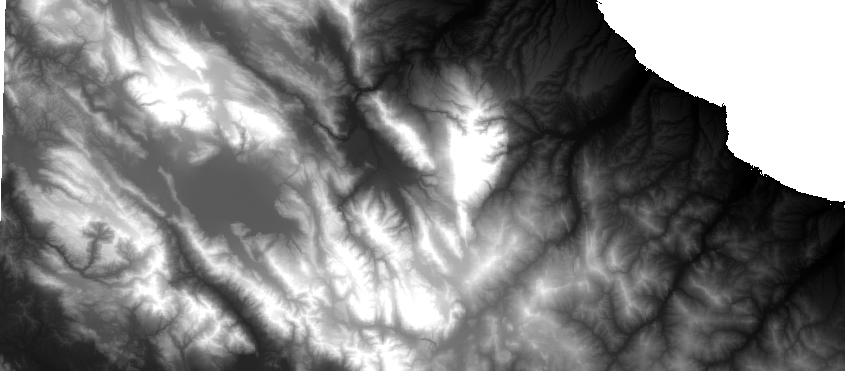
\includegraphics[width=1\textwidth]{images/STRM.PNG}
	\caption{Immagine raster (DEM) del territorio abruzzese.}
	\label{fig:raster_abruzzo}
\end{figure}

Lo SRTM consisteva in un sistema radar modificato che ha volato a bordo dello Space Shuttle Endeavour durante gli 11 giorni della missione STS-99 del febbraio 2000. Per acquisire i dati topografici dei dati di elevazione, il carico SRTM è stato equipaggiato con due antenne radar. Un'antenna era posizionata nello spazio di carico dello Shuttle, l'altra alla fine di un braccio di 60 metri che si estendeva dallo spazio di carico una volta che lo Shuttle era nello spazio. La tecnica impiegata è conosciuta come Interferometric Synthetic Aperture Radar. \newline I modelli di elevazione ricavati dai dati dello SRTM vengono usati nei Geographic Information System (GIS). Possono essere liberamente scaricati tramite internet ed il loro formato di file è supportato da molti software. Sono stati prelevati i dati raster della regione Abruzzo e attraverso QGIS (Software per la visualizzazione e l'elaborazione di dati geografici) sono state generate le curve di livello (Appendice \ref{ch:dem_to_isoipse}). Tali curve hanno una risoluzione di 25m (Figura \ref{fig:curve_di_livello}).

\begin{figure}[h]
	\centering
	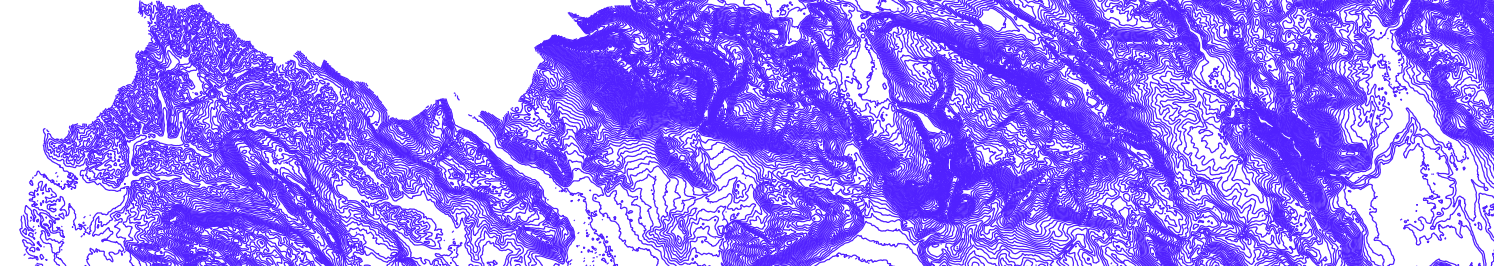
\includegraphics[width=1\textwidth]{images/dettaglioCurve.PNG}
	\caption{Curve di livello di una porzione di territorio della regione Abruzzo}
	\label{fig:curve_di_livello}
\end{figure}

Avendo introdotto le curve di livello (Isoipse) si sono decisi i valori di $Sz_k$ tenendo conto della morfologia effettiva del terreno. 
Per far ciò si è semplicemente contato il numero di curve di livello che intersecano ogni \textit{Zone}. Più il numero di intersezioni è elevato maggiore sarà la ripidità del suolo e quindi aumenterà il pericolo di frana. Il dataset ottenuto rimarca, attraverso gli \textit{Szk}, l'andamento del terreno (Figura \ref{fig:dataset_it_2}).

\begin{figure}[H]
	\centering
	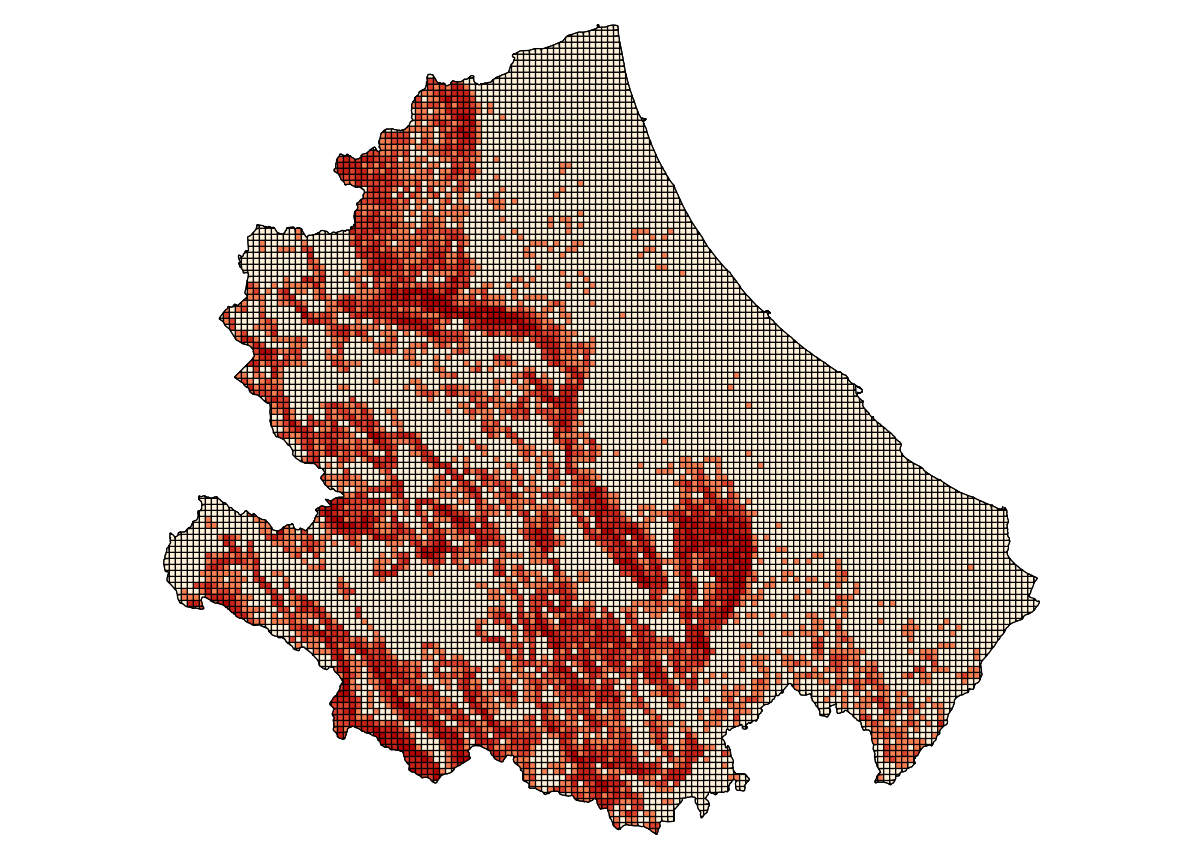
\includegraphics[width=1\textwidth]{images/abruzzoZKquadretto.png}
	\caption{Dataset ottenuto tenendo conto delle curve di livello}
	\label{fig:dataset_it_2}
\end{figure}


\subsection{\textbf{Iterazione 3}}

Nell'iterazione 2 sono emerse due problematiche di cui tener conto:

\begin{enumerate}
	\item aree estremamente piccole lungo i bordi
	\item estrema regolarità delle \textit{Zone}
\end{enumerate}

Queste problematiche sono state superate cambiando il modello di generazione delle \textit{Zone}. E' stata pertanto utilizzata la decomposizione di Voronoi. In matematica, un diagramma di Voronoi (dal nome di Georgij Voronoi), anche detto tassellatura di Voronoi, decomposizione di Voronoi, o tassellatura di Dirichlet (dal nome di Lejeune Dirichlet) è un particolare tipo di decomposizione di uno spazio metrico determinata dalle distanze rispetto ad un determinato insieme discreto di elementi dello spazio (ad esempio, un insieme finito di punti). 
Il risultato ottenuto combinando la decomposizione di Voronoi con le curve di livello ha prodotto un risultato davvero soddisfacente. Il limite delle geometrie regolari si è superato in quanto tale tassellatura genera geometrie tutte differenti tra di loro. Mentre il limite delle aree molto piccole sui bordi non si presenta affatto.
Per aumentare la variazione $Sz_k$ per le zone pianeggianti si è deciso di aggiungere un valore casuale (Figura \ref{fig:final_dataset_it_3}).

\begin{figure}[h]
	\centering
	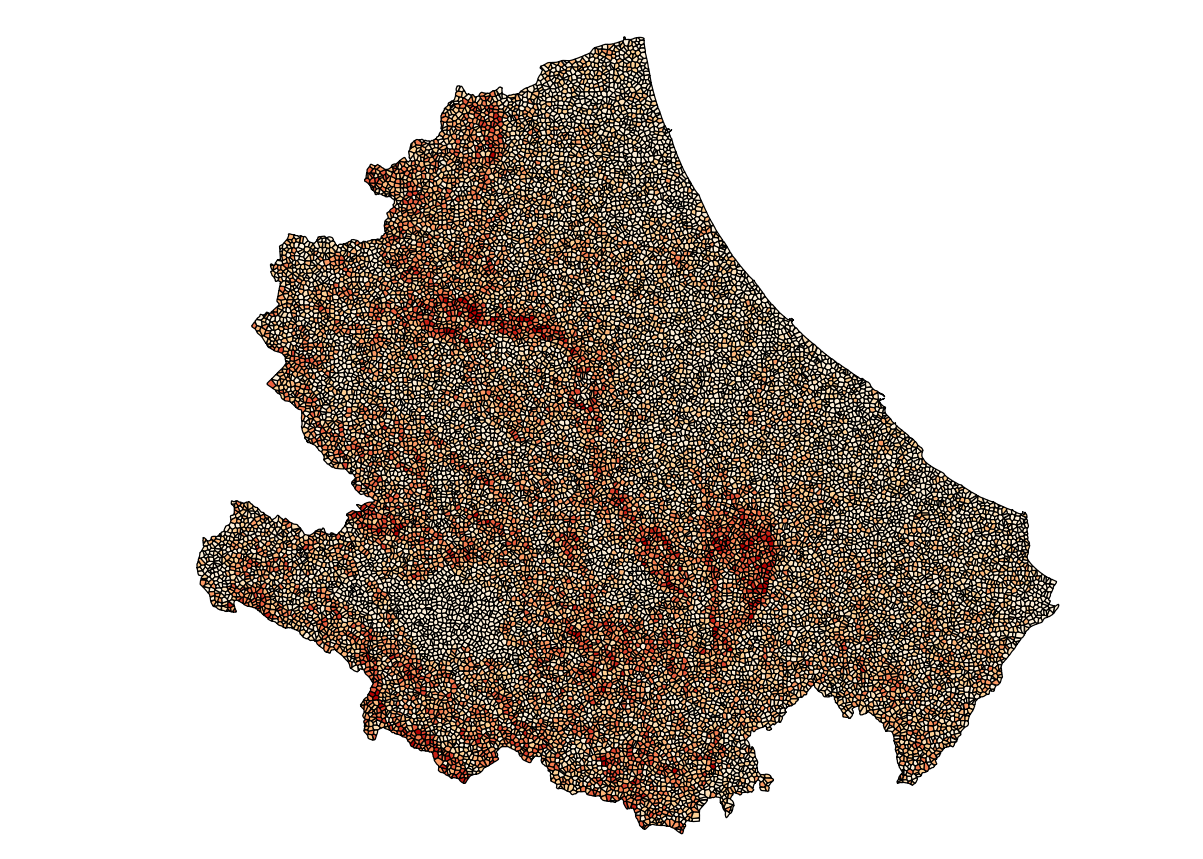
\includegraphics[width=1\textwidth]{images/voronoi.png}
	\caption{Dataset ottenuto tenendo conto delle curve di livello ed applicando la scomposizione di Voronoi}
	\label{fig:final_dataset_it_3}
\end{figure}

In definitiva attraverso le curve di livello ricavate dai dati raster, la suddivisione in poligoni di Voronoi si è ottenuto un dataset sintetico che va a rispettare tutte le specifiche che ci eravamo imposti. Di seguito viene proposta l'UDF relativa alla creazione del dataset $\mathcal{Z}$.

\newpage
\begin{lstlisting}[style = mystyle]
 CREATE TABLE voronoi AS
	SELECT (ST_DUMP(geom_voronoi)).geom AS geom_dump 
	FROM (
		SELECT ST_collectionextract(
			ST_voronoipolygons(geom_point),3) AS geom_voronoi
		FROM (
			SELECT ST_GeneratePoints( geom , 22000) AS geom_point
			FROM geo_area AS query3 
		) AS query2
	) AS query;

	CREATE TABLE dataset AS
	
	SELECT ST_Intersection(abruzzo.geom,voronoi.geom_dump) AS geom
	FROM voronoi, geo_area AS abruzzo;

\end{lstlisting}

\newpage
\begin{lstlisting}[style = mystyle]
 CREATE OR REPLACE FUNCTION zkcalcolus (idc INTEGER) RETURNS void
 LANGUAGE plpgsql
 AS $$
 DECLARE
	max INTEGER;
	min INTEGER;
	probabilita FLOAT;
	diff FLOAT;
	cursore RECORD;
	posneg FLOAT;
	variance FLOAT;
 BEGIN
 
 	--- Per ogni zone nell'insieme Z
	FOR cursore in SELECT id,geom FROM dataset WHERE idc = id LOOP
		max := 0;
		min := 0;
		diff := 0;
		probabilita := 0;
		posneg := 0;
		variance := 0;

		CREATE TEMP TABLE intersezioneQuadratino (
			id SERIAL PRIMARY KEY, 
			elevation float, 
			geom geometry
		);
	
		--- Prende tutte le curve di livello che intersecano la zone
		INSERT INTO intersezioneQuadratino(elevation, geom) 
			SELECT 
				isoipseabruzzo25.elevation,
				st_collectionextract(st_intersection(
						dataset.geom,
						isoipseabruzzo25.geom)
				,2) 
			FROM isoipseabruzzo25,dataset
			WHERE dataset.id = cursore.id;

		CREATE TEMP TABLE intersezioneQuadratinoPulita (
			id SERIAL PRIMARY KEY, 
			elevation float, 
			geom geometry);
		
		--- Scarta tutte le curve di livello con geometria nulla
		INSERT INTO intersezioneQuadratinoPulita 
			SELECT * 
			FROM intersezioneQuadratino 
			WHERE st_astext(geom) <> 'MULTILINESTRING EMPTY';

		max :=( SELECT elevation 
				FROM intersezioneQuadratinoPulita 
				ORDER BY elevation DESC LIMIT 1);
		min :=( SELECT elevation 
				FROM intersezioneQuadratinoPulita 
				ORDER BY elevation ASC LIMIT 1);

		DROP TABLE intersezioneQuadratino;
		DROP TABLE intersezioneQuadratinoPulita;

		--- L'algoritmo deve sommare o sottrare un valore casuale 
		--- all' Sz_k. Posneg serve appunto per sommare o sottrare 
		posneg :=(SELECT random());
		
		IF posneg > 0.5 THEN
			posneg = 1;
		ELSE
			posneg = -1;
		END IF;

		--- Valore randoma che vado a sommare o sottrarre un valore causale.
		variance := (SELECT (random()*0.3));
		
		variance := variance * posneg;
		diff := max - min;
		
		--- Calcola l'Sz_k
		IF diff <> 0 THEN
			IF diff > 800 THEN
				probabilita := 1;
			ELSE
				probabilita := diff / 800 ;
				probabilita := probabilita + variance;
				
				--- Questo blocco if impedisce di avere Sz_k maggiori di 1
				--- oppure minori di 0 dopo la somma con la varianza
				IF probabilita > 1 THEN
					probabilita := 1;
				END IF;
				IF probabilita < 0 THEN
					probabilita := 0;
				END IF;
			END IF;
		ELSE
			probabilita := 0;
		END IF ;
		UPDATE dataset SET zk = probabilita WHERE id = cursore.id;
	END LOOP;
END;
$$
\end{lstlisting}
